%!TEX root = ../Masterthesis.tex
\chapter{Digital hand models}
After retrieving all needed data from the real world counterpart and calculation for pose estimation is finished, the returned solution has to be displayed in the digital world. Therefore a digital hand model is needed to represent the calculated data. Modern day computer animation techniques make it possible to create nearly photo realistic digital replicas of human skin wrapped onto anatomically precisely modeled body parts. These highly complex models acquire a lot of calculation resources and are mostly not appropriate for a mealtime rendering approach.\\
When adapting calculation data to digital hand models, those of lesser complexity are preferred, sacrificing the quality of the resulting output for speed and more fluent motion results.
\begin{figure}[H]
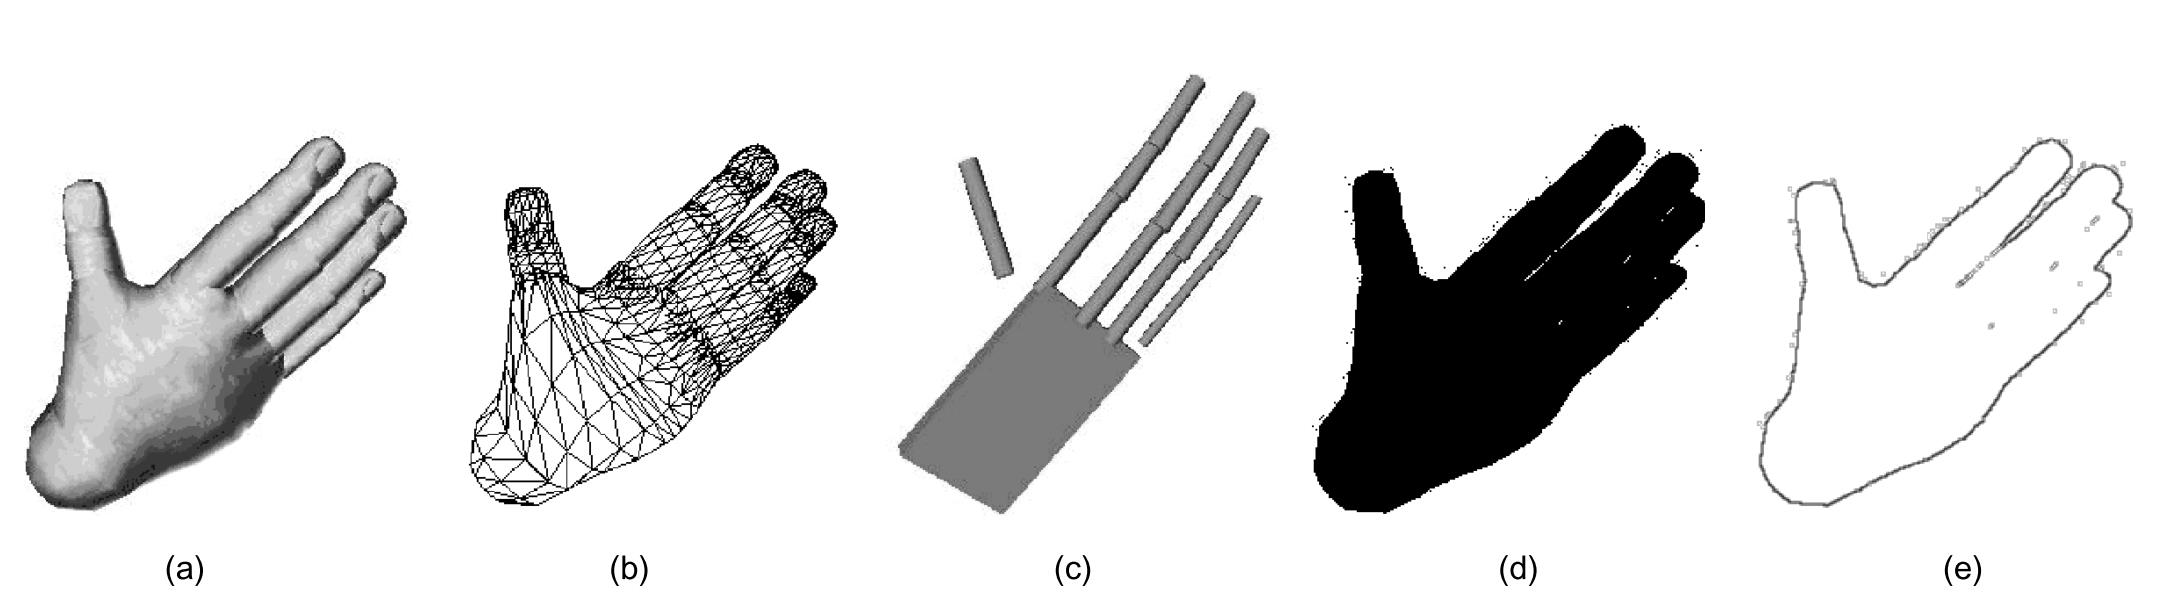
\includegraphics[width=\textwidth]{images/Pavlovic-Sharmaetal.jpg}
\caption{Pavlovic, Sharma et al: Hand models. Different hand models can be used to represent the same hand posture. (a) 3D Textured volumetric model. (b) 3D wire frame volumetric model. (c) 3D skeletal model. (d) Binary silhouette. (e) Contour.}
~\cite[p.~682]{Pavlovic.1997}
\label{handmodels_detail_level}
\end{figure}
Figure \ref{handmodels_detail_level} shows different model representations of the same hand posture. The models of \textbf{(a)}and \textbf{(b)} represent the aforementioned types of models that would be used in modern computer-graphics for displaying hand models realistically.\\These models are based on complex 3D surfaces like \textit{NURBS}(nonuniform rational B-splines) which are wrapped around an underlying skeleton. The wire frame model of \textbf{(b)} give a good overview of how many vertex calculation have to be made for the surface in each frame, causing these models to hardly run in real time if not supplying a large amount of computational power.\\
In applications where the 3D orientation of each individual finger is not necessary for processing and the general silhouette is sufficient (e.g general hand position tracking or sign language detection), even more reduced representation forms like \textbf{(d)} and \textbf{(e)} can be chosen.
The model displayed in \textbf{(c)} is a simplification of the human hand structure with geometric primitives like cylinders and boxes. These geometric primitives have the virtue of being much easier to describe than a \textit{NURBS} model. A cylinder for example is fully described by its height and its radius under the assumption that the position and orientation data is generally needed for all the described models.This type of model is also refereed to as \textit{skeletal models} as they mostly try to reproduce the strucutre of the human hand as described in Section \ref{sec:Physiological_structure_of_the_human_hand}





